\section{Introduction}

%\par
%(1) Keep the section 1 (context, problematic).

In many contexts (e.g. industry, academic research, etc.), users want to get insights about their data. In such cases, the number of features characterizing each instance in their dataset is often too large to understand their data. The problem of {\it dimensionality reduction} (DR) is to reduce a dataset containing $D$ features for $N$ instances (providing an $N \times D$ matrix) to a new dataset of $Z$ dimensions, such that $Z \ll D$. When this new number of dimensions $Z$ equals two, the dimensionality reduction result allows users to see their data in a two-dimensional space by plotting the remaining two dimensions in a scatter plot. This problem is called {\it visualization}: from provided data with too many features, visualization algorithms provide a projection of these data in a two-dimensional space in such a way that the information loss is minimized. The resulting $N \times 2$ matrix, often called {\it embedding}, can then be visualized.
% For instance, Fig.~\ref{subfig:digit_viz_example} represents a visualization of 200 hand-written digits images from the well-known MNIST dataset and Fig.~\ref{subfig:digit_example} shows some examples of the raw image data.

% \begin{figure}[!htb]
%     \centering
%     \begin{subfigure}[c]{0.45\linewidth}
%         \frame{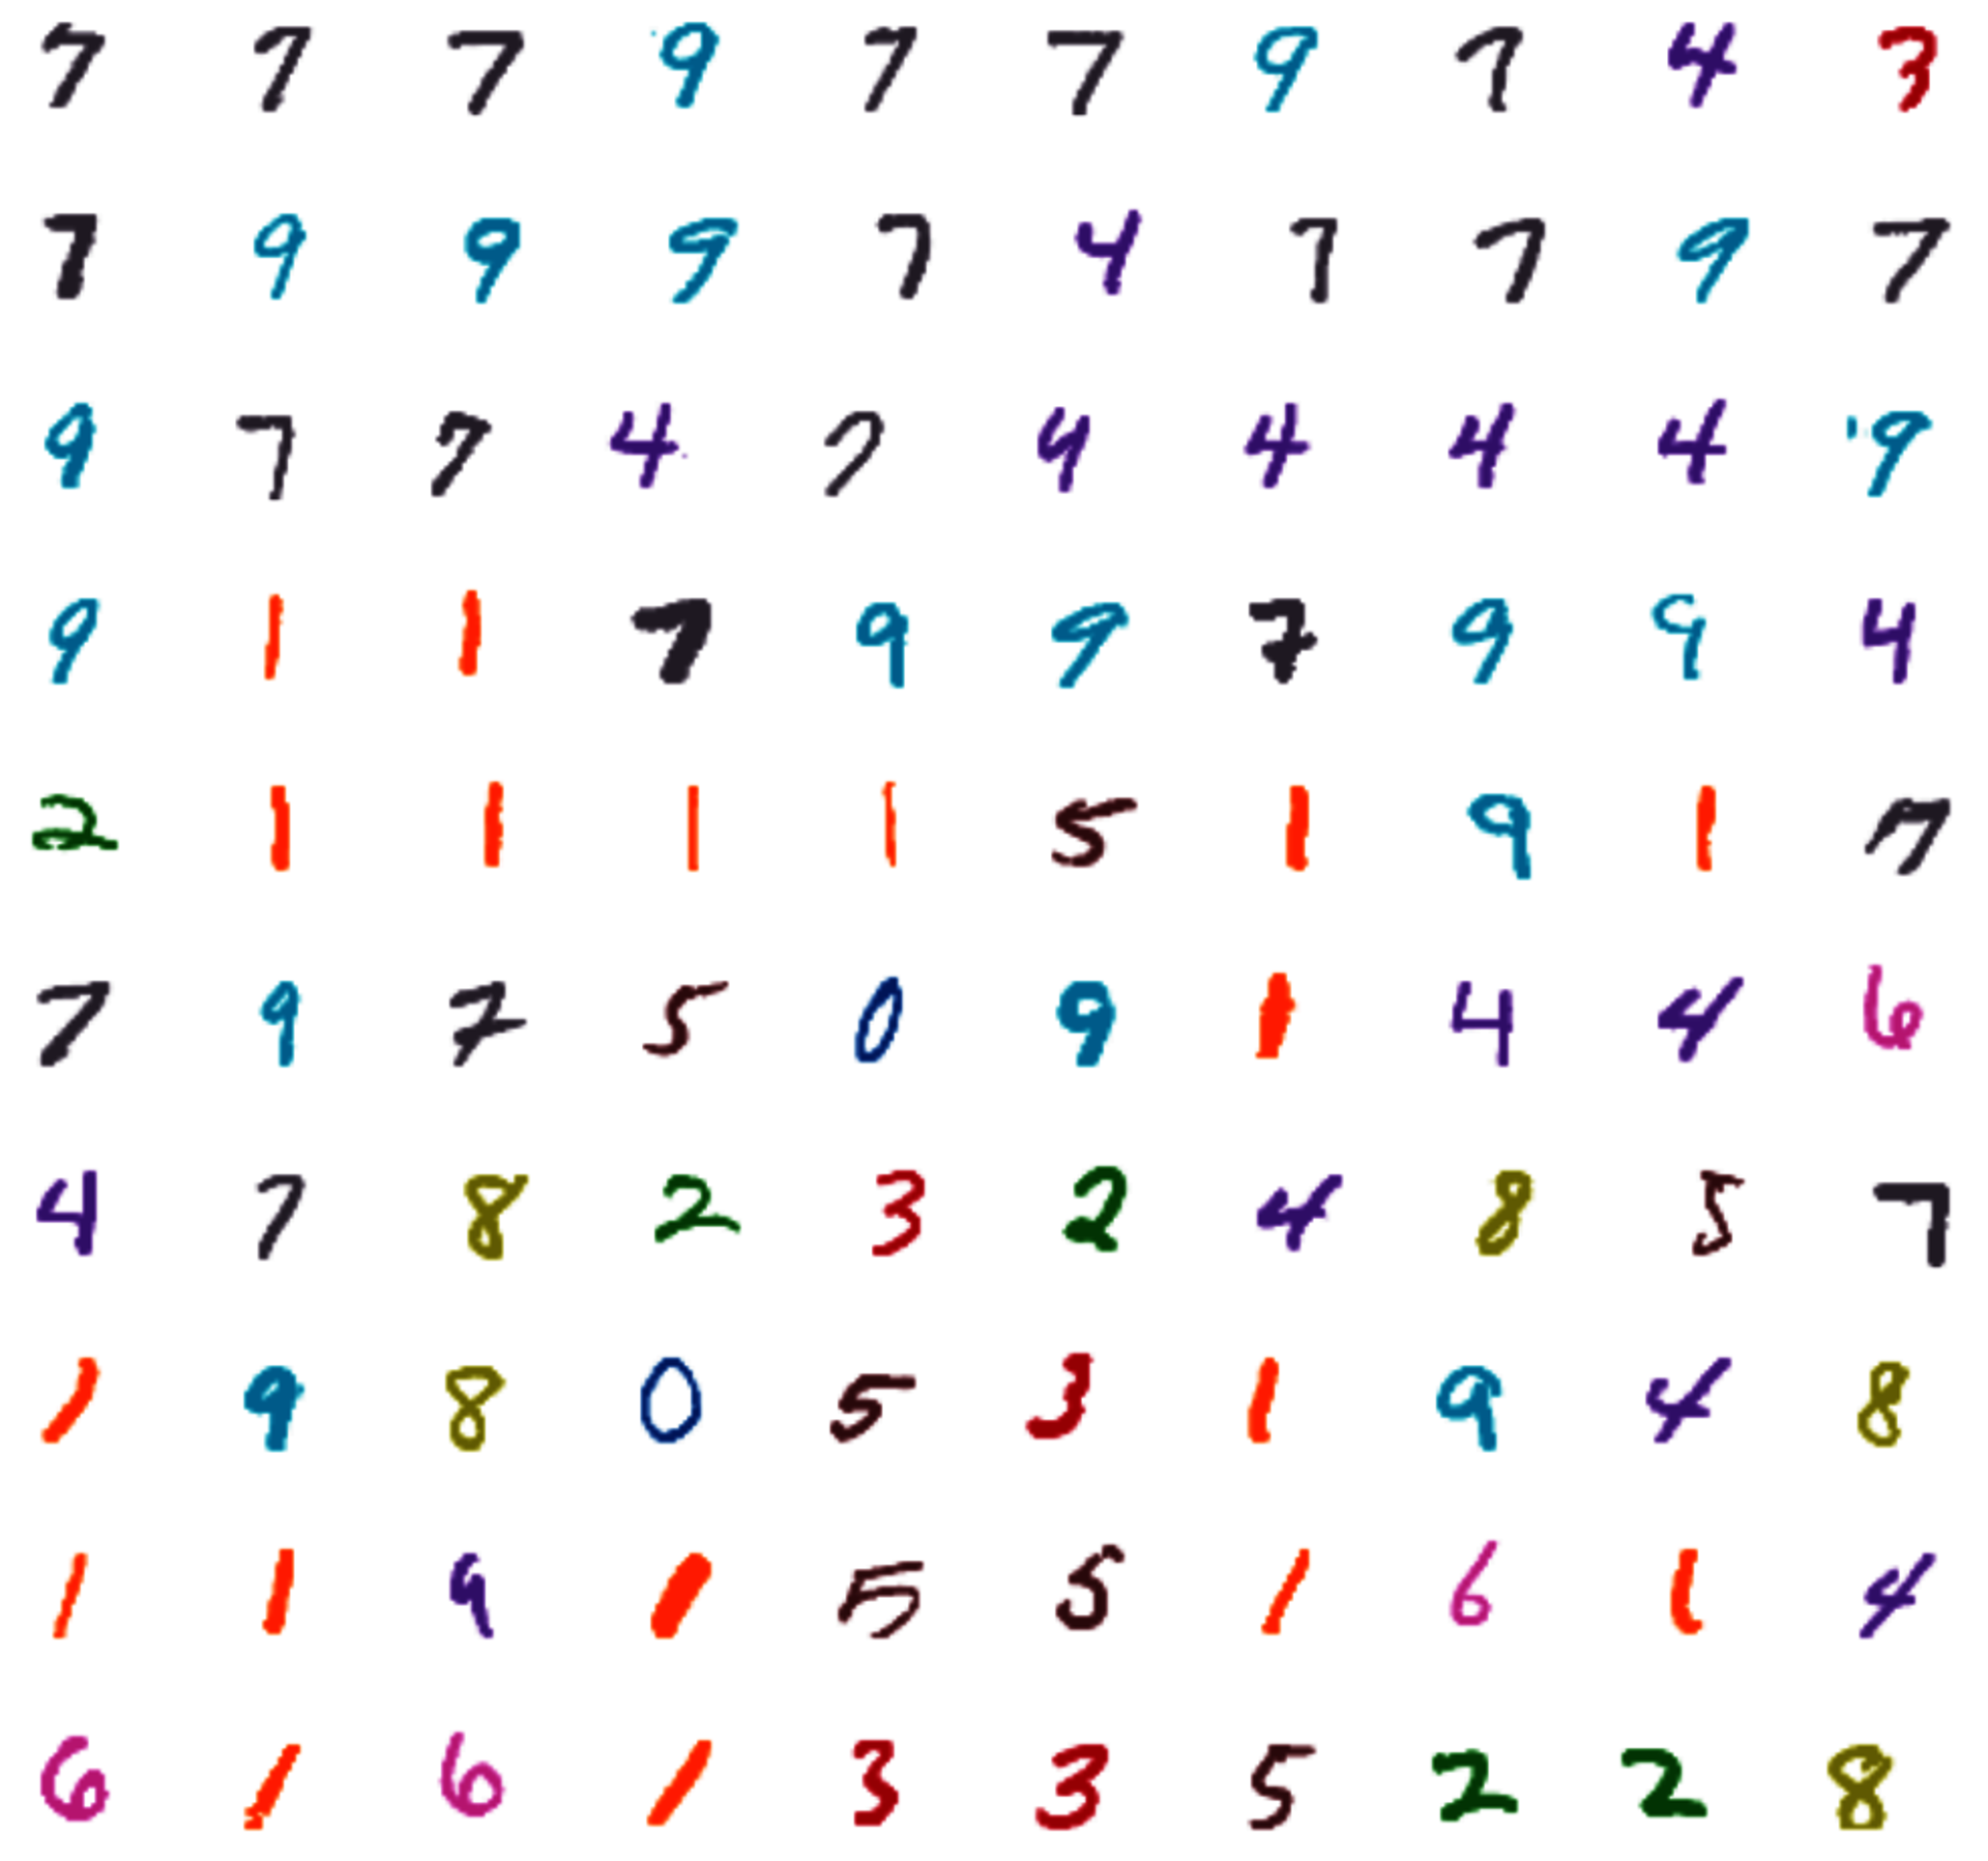
\includegraphics[width=\textwidth]{figures/mnist_raw200}}
%         \caption{Examples of hand-written digit images.}
%         \label{subfig:digit_example}
%     \end{subfigure}
%     \begin{subfigure}[c]{0.53\linewidth}
%         \frame{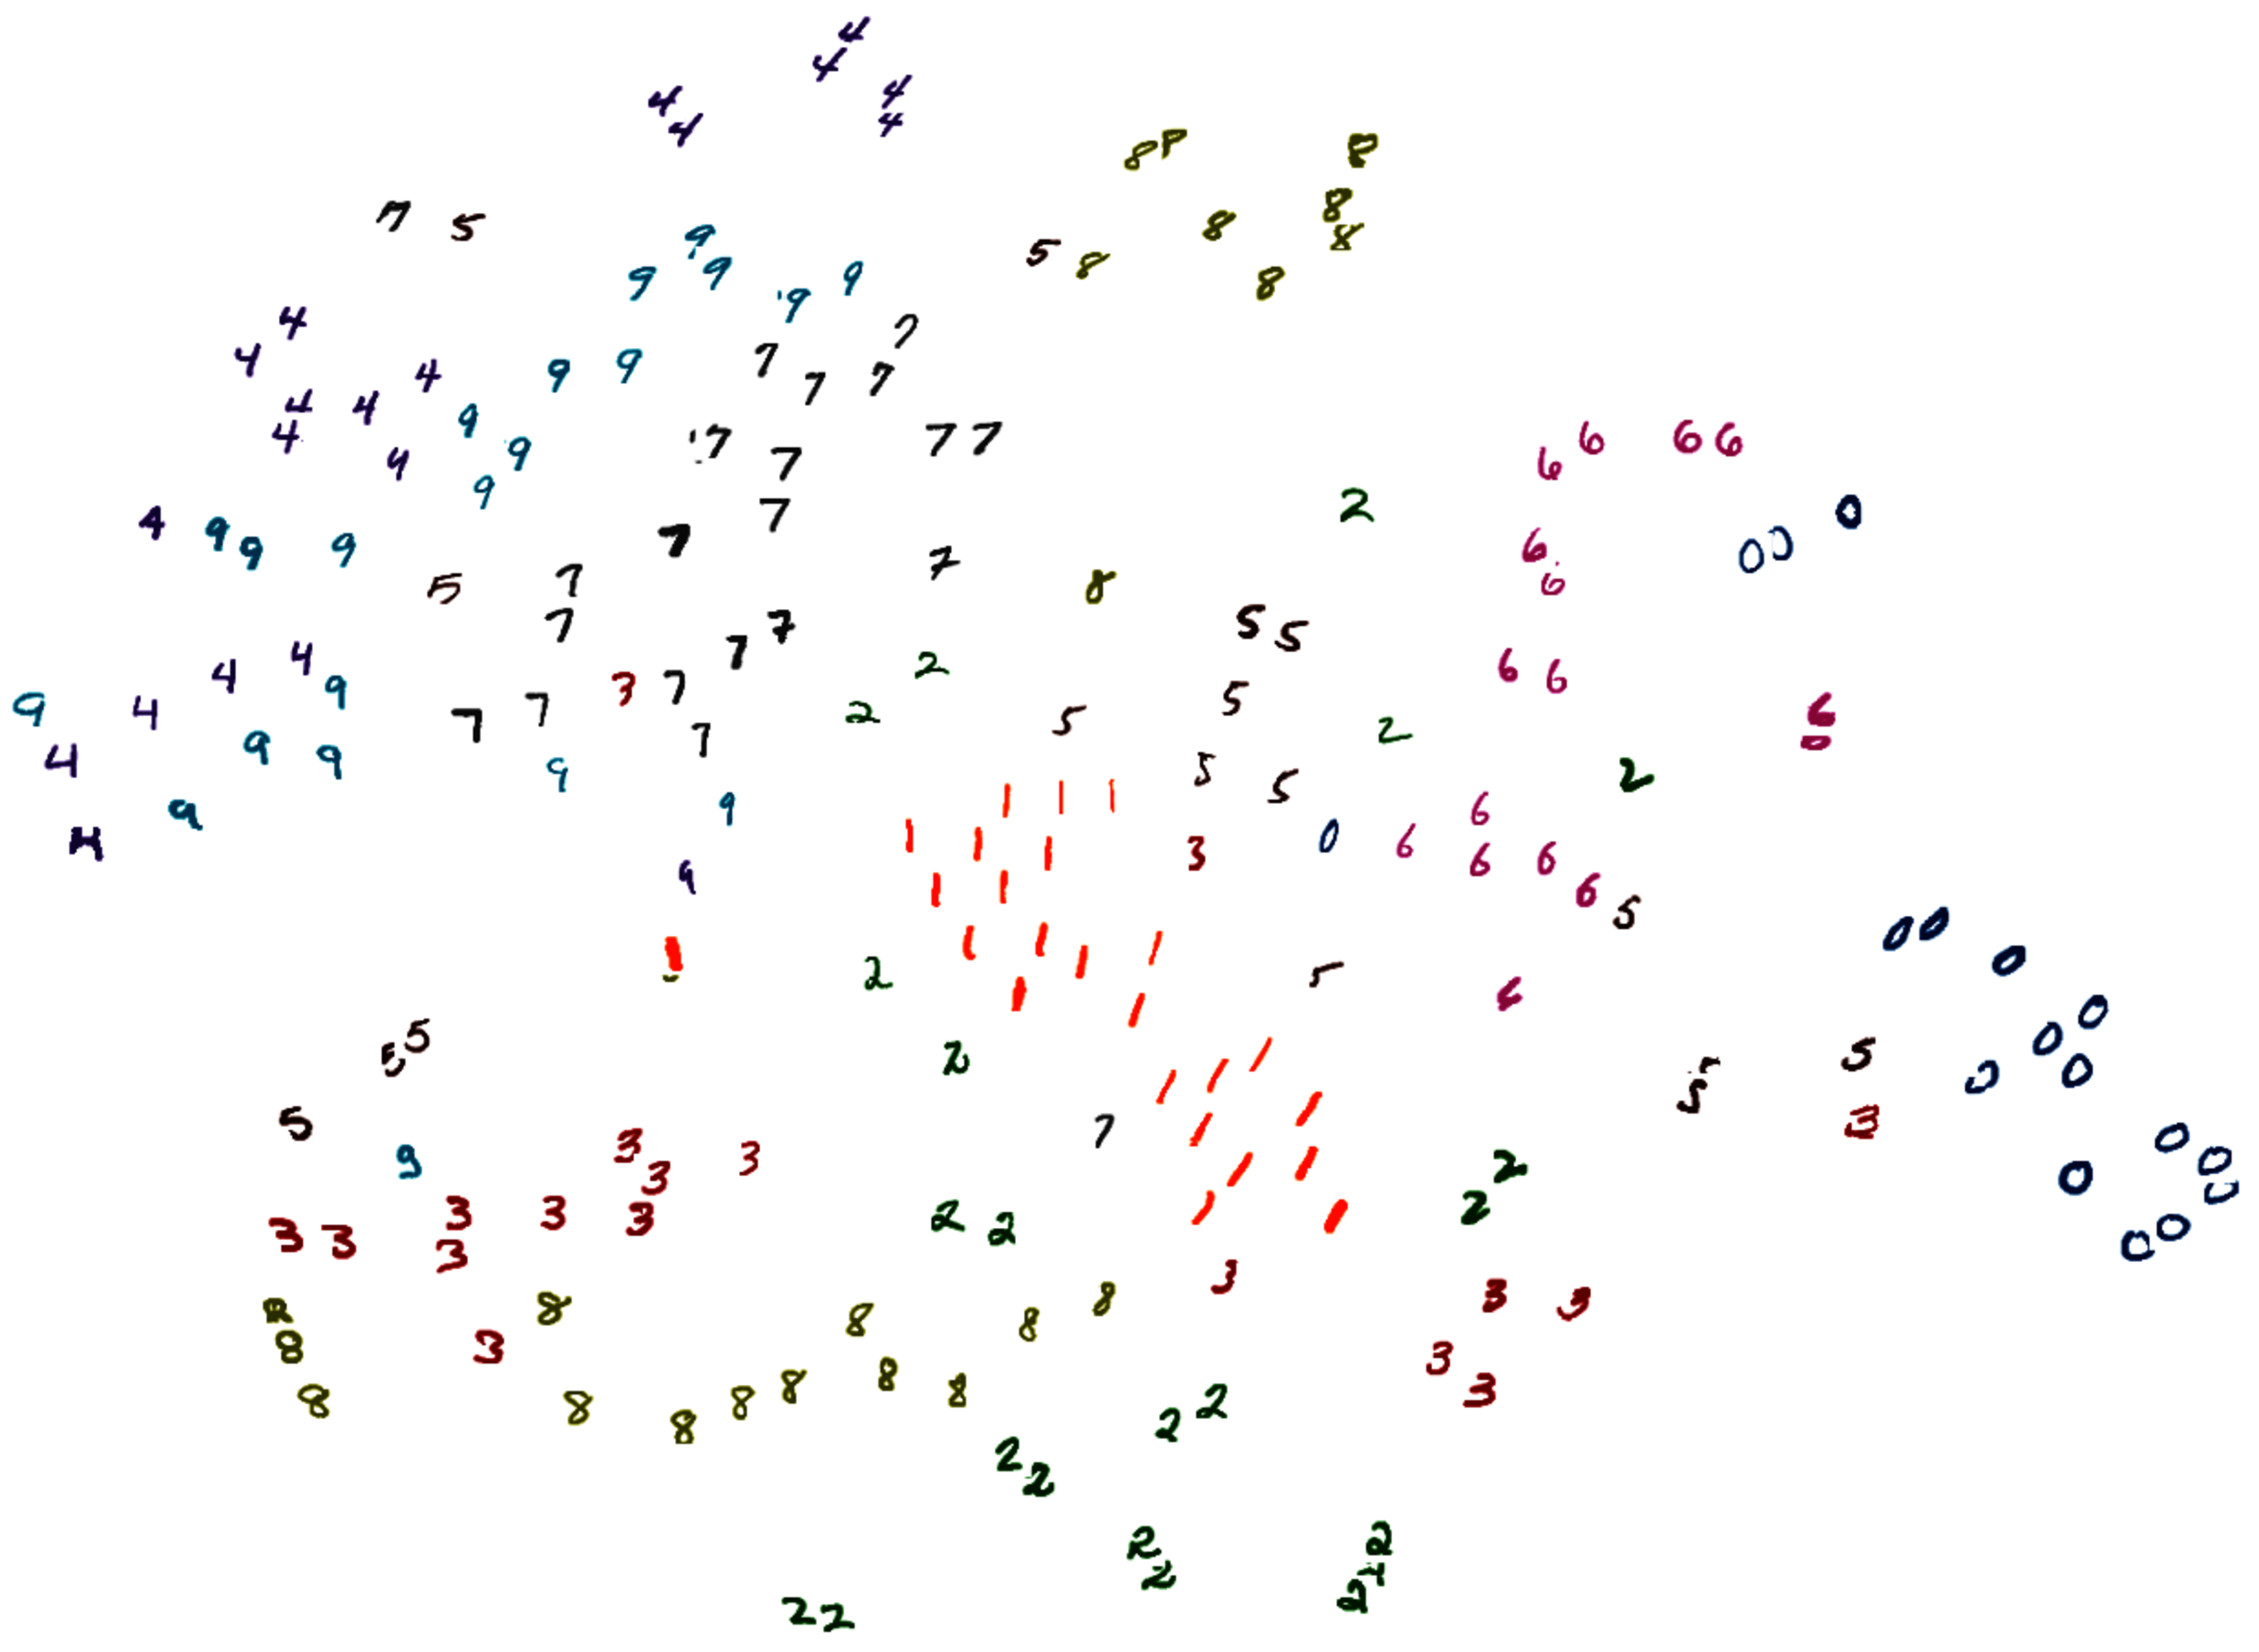
\includegraphics[width=\textwidth]{figures/mnist_viz200}}
%         \caption{A visualization created by \mbox{$t$-SNE}.}
%         \label{subfig:digit_viz_example}
%     \end{subfigure}
%     \caption{Example of 32x32 images of hand-written digits which are visualized by a dimensionality reduction technique ($t$-SNE) and represented in a 2D scatter plot.}
%     \label{fig:dr_viz}
% \end{figure}

Some DR visualization algorithms require to tune one or more hyperparameters (e.g. $t$-SNE~\cite{maaten2008tsne}, LargeVis~\cite{tang2016visualizing} and UMAP~\cite{mcinnes2018umap}). This step is crucial, since it predetermines the quality and usefulness of the obtained visualization. Typically, the desired visualization result has to be chosen through trial and error by the user among all generated results using different hyperparameter values. This process is tedious, which makes it difficult for the user to find the best suiting visualization.

\begin{figure*}%[h]
  \centering
  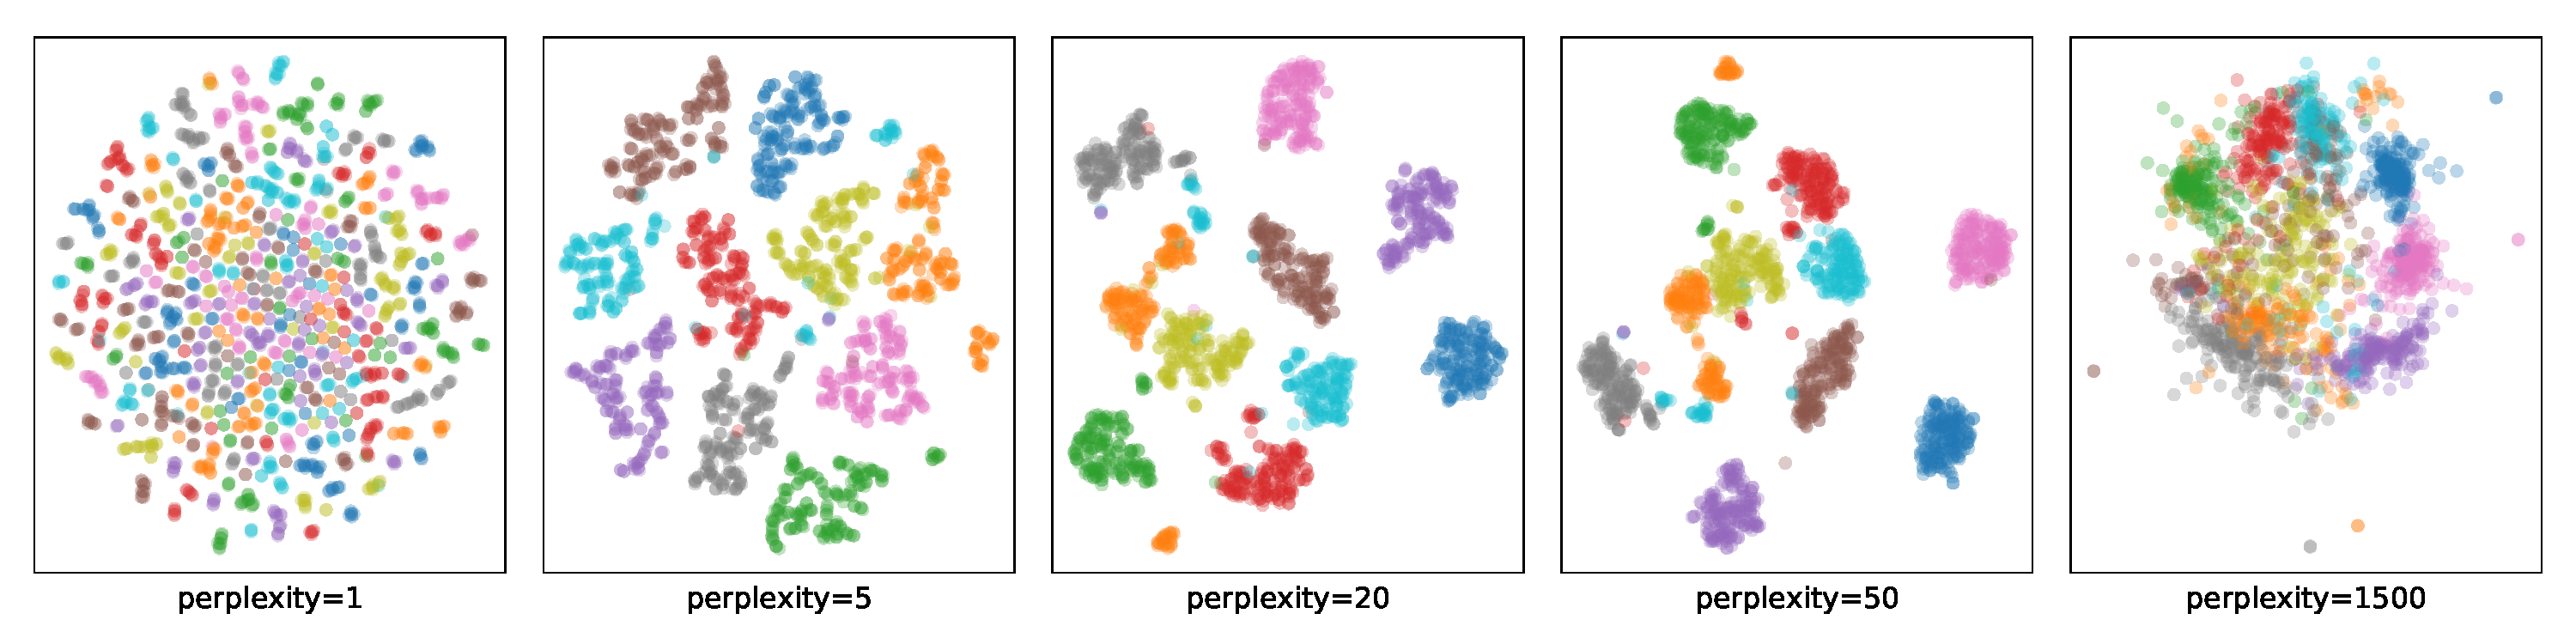
\includegraphics[width=\linewidth]{figures/MNIST-SMALL_examples}
  \caption{Visualization of the \emph{DIGITS} dataset by $t$-SNE with five different perplexity values preserving the local (left) to global (right) topology of the dataset. The dataset contains 1797 gray-scale 8x8 images representing ten different handwritten digits. The colors correspond to these different digits. Perplexities of 1 and 1500 are extreme results showing that points have one or a couple of neighbors (perplexity = 1) or they have nearly all instances in the dataset as neighbors (perplexity = 1500). Obtaining compact clusters (perplexities of 20 and 50) is usually considered better.}
  \label{fig:mnist_perps}
\end{figure*}

In this paper, we show how to automatically choose the hyperparameters of DR techniques, such as the {\it perplexity} of $t$-SNE, by considering pairwise constraints.
% We propose to consider user constraints on the dataset of interest to maximize the chance for the most suitable visualization to be presented to the user.
The constraints are in form of relationships between object pairs, which are easier to express and understand for users. These user pairwise constraints are first transformed into a quantitative measure called \emph{constraint-preserving score} and then used to find a range of hyperparameter values corresponding to the best visualizations that respect the user needs. A Bayesian optimization approach~\cite{mockus1974BO, mockus1978application} is used to find this range.

The approach of finding the best hyperparameter values with an external score, instead of modifying the chosen DR methods, allows us to apply the technique to any kind of DR methods. In that sense, the approach is DR-method-agnostic. Furthermore, our approach is a step towards the automatization of the ML pipeline (AutoML) in the context of DR, while preserving explainability. Indeed, when using the constraint for choosing the best hyperparameter values, visualizing these constraints makes it possible to explain the choice of visualization. This may ease the use of DR methods by end-users to visualizes their own data without caring about the complex algorithms and hyperparameters. Indeed, end users can use our method as a black-box hyperparameter tuning toolbox. Furthermore, the approach can also be used by DR experts to analyze the impact of hyperparameters on the quality of visualizations.

%%%%%%%% Outline of the paper
%%%%%%%%%%%%%%%%%%%%%%%%%%%%%%%%%%%%
This paper is organized as follows. Section~\ref{sec:background} presents the background on dimensionality reduction, visualization quality metrics and pairwise constraints in unsupervised learning, and provides an overview of how the automatic hyperparameter selection of DR methods is handled in the literature. Our proposed method, which takes constraints into account in order to select the best set of hyperparameter values, is introduced in Section~\ref{sec:proposed_method}. The experimental setting for evaluating our proposed method is described in Section~\ref{sec:xp:setup}. The results that are presented in Section~\ref{sec:results} and discussed in Section~\ref{sec:discussion}. Finally, Section~\ref{sec:conclusion} concludes our work.

%%%%%%%%%%%%%%%%%%%%%%%%%%%%%%%%%%%%%%%%%%%%%%%%%%%%%%%%%%%%%%%%%%%%%%%%%%%%%%
\section{Background and Related Work}\label{sec:background}

This section presents the background and methods related to our work. Dimensionality reduction techniques that are used in our evaluation (i.e $t$-SNE, UMAP and LargeVis) are presented in Section~\ref{subsec:background_DR}. Quality measures that are used in the literature to characterize the quality of DR embeddings are presented in Section~\ref{subsec:qual_metrics_background}. The use of user constraints in clustering and in DR is presented in Section~\ref{subsec:user_constraints_clustering_DR}. Finally, the techniques to choose hyperparameters for DR algorithms are reviewed in Section~\ref{subsec:tune_HP}.%, and the way to tune it with Bayesian optimization is presented in Section~\ref{subsec:tune_with_BayOpt}.

\subsection{Dimensionality Reduction for Visualization}\label{subsec:background_DR}

Dimensionality reduction (DR) is an unsupervised learning problem in machine learning with the goal of reducing the number of dimensions of a multivariate dataset while preserving its important characteristics. In the specific case of a lower-dimensional space of two dimensions, the instances in this new space can be visualized. Typical characteristics that DR visualization techniques try to preserve are variance (as in PCA), similarities and distances between objects (distance-preserving, as in MDS), or cluster structures and neighborhood information among objects (neighborhood preservation, as in $t$-SNE) \cite{lee2007}. Three DR visualization techniques containing one or more hyperparameters are used for comparison in this paper: $t$-SNE, UMAP and LargeVis.

$t$-distributed Stochastic Neighbor Embedding ($t$-SNE)~\cite{maaten2008tsne}, one of the most widely used DR method, preserves the neighborhood information by creating an embedding in such a way that the points that are neighbors in the original high-dimensional space (HD) will still be neighbors in the reconstructed low-dimensional space (LD). 
The number of neighbors to consider for each point (controlled by the \emph{perplexity} hyperparameter) is usually determined by the user.
Fig.~\ref{fig:mnist_perps} shows some visualizations generated with different perplexities. 
It can be seen in the figure that the structure in each visualization changes according to the considered number of neighbors for each point, defined by the perplexity. When the perplexity is very small, small local groups/clusters of points appear. These groups become more and more large and compact when the perplexity increases, meaning that more neighbors for each point are preserved. However, when the perplexity is too large, each point is considered as neighbor of every other point, which leads to a crowded ball-shaped cluster. This evolution is a specific characteristic of the neighborhood-preserving DR methods. In order to use $t$-SNE efficiently, the user is required to have a good knowledge of the dataset for choosing a reasonable perplexity, as well as for interpreting and analyzing the visualization.

In the literature, the classical distance-preserving DR techniques are not always efficient because they cannot fully retain both global and local structure of the high dimensional data \cite{maaten2008tsne, van2009comparativeReview}. $t$-SNE tackles this problem by transforming the pairwise distances in HD and LD into probabilities. The intuition behind this probability-preserving approach is as follows.
Let us assume that the original data in HD is modeled by a distribution $P$ and the reduced data in LD is modeled by a distribution $Q$.
These two distributions represent the probability of being neighbors for each pair of points in HD and LD respectively.
The objective of $t$-SNE is to minimize a measure called the Kullback-Leibler (KL) divergence loss by seeking an embedding whose distribution $Q$ comes closer and closer to the true distribution $P$~\cite{maaten2008tsne}:

\begin{equation}\label{eq:p_j|i}
    p_{j|i} = \frac{\textnormal{exp}(-||x_i - x_j||^2/2\sigma_i^2)}{\sum_{k\not=i}\textnormal{exp}(-||x_i - x_k||^2/2\sigma_i^2)}
\end{equation}

\begin{equation}
    p_{ij} = \frac{p_{j|i}+p_{i|j}}{2}
\end{equation}

\begin{equation}\label{eq:q_ij}
    q_{ij} = \frac{(1+||y_i - y_j||^2)^{-1}}{\sum_{k\not=l}(1+||y_k - y_l||^2)^{-1}}
\end{equation}

\begin{equation}\label{eq:KL}
    KL(P||Q) = \sum_{i}\sum_{j} p_{ij} \textnormal{log}\frac{p_{ij}}{q_{ij}}.
\end{equation}

$t$-SNE is controlled by a hyperparameter called the perplexity, one of the most important  $t$-SNE hyperparameter, which approximates the number of neighbors considered for each point through $\sigma$ in Eq.~\ref{eq:p_j|i}. The user can change the perplexity to obtain different visualizations. With a small perplexity, the local structure is preserved, while a larger perplexity pays more attention to the global structure of the dataset. Tuning this parameter is a difficult task and is usually done by trial and error.

Uniform Manifold Approximation and Projection (UMAP) \cite{mcinnes2018umap} is a new DR technique that challenges $t$-SNE in terms of visualization quality. As for $t$-SNE, UMAP is based on a the notion of neighborhood preservation. The first phase of the algorithm is to build a weighted adjacency matrix ${\bf A}$ of a k-nearest neighbors graph in HD. The weight between the instance ${\bf x}_i$ and one of its closest neighbor ${{\bf x}_i}_j$ is defined as
\begin{equation}
    w(({\bf x}_i, {{\bf x}_i}_j)) = \textnormal{exp} \left( \frac{-\textnormal{max}(0, d({\bf x}_i, {{\bf x}_i}_j) - \rho_i)}{\sigma_i} \right),
\end{equation}
where $d(\cdot, \cdot)$ is a distance or dissimilarity measure, $\rho_i = \textnormal{min}\{d({\bf x}_i, {{\bf x}_i}_j) | 1 \leq j \leq k, d({\bf x}_i, {{\bf x}_i}_j) > 0\}$, and $\sigma_i$ is set such that
\begin{equation}
    \sum _{j=1}^k \textnormal{exp} \left( \frac{-\textnormal{max}(0, d({\bf x}_i, {{\bf x}_i}_j) - \rho_i)}{\sigma_i} \right) = \textnormal{log}_2(k).
\end{equation}
The UMAP's adjacency matrix ${\bf B}$ that is used for characterizing the HD neighborhoods is then computed as
\begin{equation}
    {\bf B} = {\bf A} + {\bf A}^\top - {\bf A} \circ {\bf A}^\top.
\end{equation}

In a second step, points ${\bf y}_i$ and ${\bf y}_j$ in LD, corresponding to HD points ${\bf x}_i$ and ${\bf x}_j$, are positioned in the 2D map according to \textit{attractive forces} defined by
\begin{equation}
    \frac{-2ab{||{\bf y}_i - {\bf y}_j||}^{2(b-1)}_2}{1+{||{\bf y}_i - {\bf y}_j||}^2_2}w(({\bf x}_i, {\bf x}_j))({\bf y}_i - {\bf y}_j)
\end{equation}
and \textit{repulsive forces} defined by
\begin{equation}
    \frac{b}{(\epsilon+{||{\bf y}_i - {\bf y}_j||}^2_2)(1+{||{\bf y}_i - {\bf y}_j||}^2_2)}(1-w(({\bf x}_i, {\bf x}_j)))({\bf y}_i - {\bf y}_j),
\end{equation}
where $a$ and $b$ are hyperparameters \cite{mcinnes2018umap}. The two hyperparameters that are considered for tuning in this paper are $k$, the number of neighbors considered, and min-dist, the distance between neighbors in LD, which is defined based on $a$ and $b$. 

The third DR visualization technique that is used in our evaluation is LargeVis. LargeVis has been developed to overcome the scalability problem that face many DR techniques. Indeed, with millions of instances, state-of-the-art techniques such as $t$-SNE does not work \cite{tang2016visualizing}. While the first step of LargeVis is to efficiently build a k-nearest neighbor graph in HD based on $t$-SNE $p_{j|i}$ (see Eq.~\ref{eq:p_j|i}), the second step is to match the probability that an edge $e_{ij}$ links the instances ${\bf x}_i$ and ${\bf x}_j$ in HD (i.e. they are neighbors) with the distance between the corresponding points ${\bf y}_i$ and ${\bf y}_j$ in LD:
\begin{equation}
    P(e_{ij}) = f(||{\bf y}_i - {\bf y}_j||),
\end{equation}
where $f$ is a probabilistic function \cite{tang2016visualizing}. With the generalization that an edge $e_{ij}$ takes a weight $w_{ij}$ defined by $P(e_{ij} = w_{ij}) = P(e_{ij} = 1)^{w_{ij}}$, LargeVis objective function becomes
\begin{equation}
    \sum_{(i,j) \in E} w_{ij}logp(e_{ij} = 1) + \sum_{(i,j) \in \bar{E}} \gamma log(1 - p(e_{ij} = 1)),
\end{equation}
where $\gamma$ is a weight given to non-existing edges. As LargeVis is based on the $p_{j|i}$ of $t$-SNE, the perplexity is also a hyperparameter of LargeVis.

%Now that the state-of-the-art DR visualization methods that contain hyperparameters are presented, metrics that can assess the quality of DR produced visualizations are reviewed and discussed in the next section.

\subsection{Visualization Quality Metrics}\label{subsec:qual_metrics_background}

There exist several metrics to evaluate the quality of an embedding.  
In this paper, clustering-based quality measures are not considered because they need labeled data for measurement (e.g. the digits in the dataset DIGITS).
%For these reasons, we only use cluster-label agnostic metrics.
We also avoid quality measures that are linked to the objective function of SNE, e.g. Neighborhood Retrieval Visualizer (NeRV) \cite{venna2010}, (i) because they need the evaluation of their own perplexity parameter and (ii) because of the bias of measuring the quality of $t$-SNE and LargeVis with a quality metric too closely related to SNE.

\begin{table}%[width=\textwidth,cols=6,pos=h]
\caption{Properties of the five cluster-label-agnostic quality metrics considered in this paper to assess visualizations.}\label{tab:metrics}
\begin{tabular}{p{1.5cm} p{0.8cm} p{4.5cm}}
\toprule
Metric name &  Range value & Description\\
\midrule
CC & $[0, 1]$ & Pearson correlation coefficient between pairwise distance vectors\\
NMS & $[0, +\infty[$ & Stress based on comparison of pairwise distance orders\\
CCA & $[0, +\infty[$ & Stress with emphasis put on LD\\
NLM & $[0, +\infty[$ & Stress with emphasis put on HD\\
AUC$_{log}$RNX & $[0, 1]$ & How neighbors in HD are preserved in LD\\
\bottomrule
\end{tabular}
\end{table}

Five metrics have been selected for evaluating the quality of visualizations. 
The first considered metric, the \emph{correlation coefficient} (CC)~\cite{geng2005}, compares the pairwise distances in the HD and LD spaces by computing the correlation between the distance vectors in HD and LD. The well-known \emph{Kruskal's non-metric stress} (NMS)~\cite{kruskal1964}, often used as objective function of non-metric multidimensional scaling, is used to compare the pairwise distance orders between the high and low-dimensional space. The \emph{curvilinear component analysis stress}~(CCA) \cite{demartines1997} is a kind of Kruskal's stress with an emphasis on the embedding pairwise distances. The metric evaluates the embedding quality by looking whether if instances in the low-dimensional space are close to each other. The \emph{Sammon's non-linear mapping stress}~(NLM)~\cite{sammon1969}, is a measure similar to CCA, but focusing on the closeness of instances in the high-dimensional space. Finally, the \emph{AUC$_{log}$RNX}~\cite{lee2015} compares the neighborhood of each instance in the high and low-dimensional spaces for all possible neighborhood sizes. Table~\ref{tab:metrics} summaries these metrics and mathematical details are provided in Appendix A. 

\subsection{User Constraints for Clustering and DR}\label{subsec:user_constraints_clustering_DR}

Clustering is a machine learning problem in which the goal is to find groups (called \emph{clusters}) of instances in the data. The constraints used in clustering methods have been well studied for a long time. User constraints can incorporate domain expertise with the goal of explicitly defining the property of the expected clusters.
The popular survey by Davidson et al.~\cite{Davidson2007surveyClt} focuses on \emph{constraint-based} and \emph{distance-based} clustering methods with instance-level constraints.
In constraint-based methods, the clusters are formed in such a way that the given constraints are preserved as much as possible, e.g. PCKMeans \cite{basu2004active} and another modified version of K-Means \cite{davidson2005clustering}. % with feasibility under different types of constraints \cite{davidson2005clustering}. %$\delta-$, $\epsilon-$ and pairwise constraints
In distance-based methods, the constraints are first used to train a distance function that is later used by a clustering algorithm (e.g. \cite{bar2003learning,xing2003distance}). %, e.g. relation component analysis as distance measure \cite{bar2003learning} and constraint metric K-Means \cite{xing2003distance}.
The pairwise constraints are first introduced in constrained K-Means by Wagstaff et al. \cite{wagstaff2001constrained}. Must-link and cannot-link constraints indicate that two instances must be in the same cluster or cannot be in the same cluster, respectively.
%A similar-link constraint suggests that two points should be close, or similar, and a dissimilar-link constraint means that two points should be far apart or dissimilar.

%\subsubsection{User Constraints for Dimensionality Reduction}\label{subsec:constraints_dr}
% TODO: link to user constraints for DR
One application of user constraints in DR methods is for visualizing data in which we can inject constraints to force the output embedding to have some expected properties.
The \emph{objective constraints} can be partial labels, as in semi-supervised LDA \cite{Sugiyama2008SELF}, or constraints on the value of features, as in bounded PCA \cite{giordani2007bpca}. 
If users can interact with the visualization result, they can give their feedback in form of instance-level \emph{subjective constraints}.
Integrating user interaction into DR methods is reviewed by Sacha et al.~\cite{Sacha2017Interaction}, and Endert et al.~\cite{Endert2017SOTA} proposes a wider survey on integrating machine learning into visual analysis.
Pairwise constraints in DR are used to attract points connected by similar-links and repulse dissimilar-link constrained points. Such constraints are used in, e.g., pairwise constraints-guided feature projection~\cite{tang2007pairwise}, semi-supervised DR~\cite{zhang2007ssdr}, graph-driven constrained DR via linear projection~\cite{davidson2009gcdr} and constrained locality preserving projections~\cite{cevikalp2008CLPP}.

The objective of this paper is to show that user-constraints can also be used for automatically tuning hyperparameters of DR methods. The next section reviews how the literature handles the choice of hyperparameter values in the context of DR methods.

\subsection{Choosing Hyperparameter Values of DR Methods}\label{subsec:tune_HP}

The value of the hyperparameter depends on the characteristics of the dataset such as the number of instances (size), the topology (structure) or the density (distribution) of instances, which makes it hard to select the best one.
Concerning $t$-SNE for instance, the original paper of van der Maaten et al. \cite{maaten2008tsne} suggests typical values between 5 and 50.
However, in practice, the embedding can change drastically between two different perplexity values. Therefore, there is no evidence to ensure that the suggested perplexities are good for all datasets.
The original paper also proposes a simple method to select a good perplexity by looking at the KL loss produced by several perplexities and choose the lowest one, since it corresponds to a well-preserved neighborhood.
However, the KL loss tends to naturally decrease when the perplexity increases \cite{cao2017automatic}, which  is confirmed by our experiments, as shown in Fig.~\ref{fig:klloss}. For this reason, it is unsuitable to use the KL loss for evaluating the embedding quality since a very high perplexity would be chosen.
In practice, users have to carefully choose a hard-to-understand perplexity to obtain a good embedding.
In addition to require an expertise in machine learning, this process is often tedious and error-prone.

\begin{figure}
    \centering
    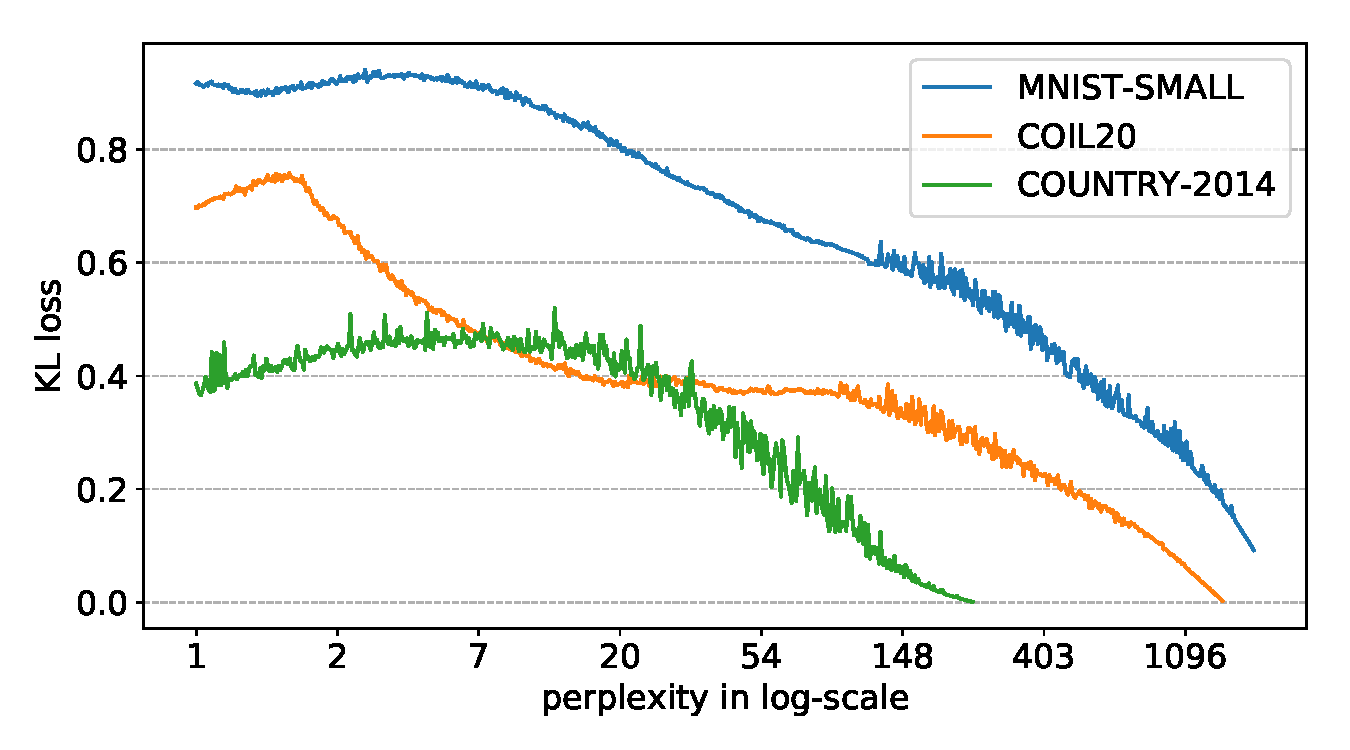
\includegraphics[width=0.95\linewidth]{klloss_all}
    \caption{For three different datasets, the KL loss tends to decrease when the perplexity increases. Note that the values of KL loss across different datasets are not comparable.}
    \label{fig:klloss}
\end{figure}

Few papers in the literature attempt to derive the best hyperparameter values automatically.
Strickert~\cite{strickert2012} avoids the burden of choosing the perplexity of $t$-SNE by evaluating the degree of neighborhood P*, instead of P, using a given pairwise score matrix S. For each instance $i$ in ${\bf S}$, all other instances $j$ are ranked and ${P}^*_{ij}$ is computed with respect to the ranking position of each instance $j$ in ${\bf S}_i$. However, this solution is not suitable when the matrix ${\bf S}$ is not provided.
Lee et al.~\cite{lee2014} use a multi-scale approach by considering, and averaging, all neighborhood sizes. Despite providing visualizations by bypassing the perplexity selection problem, these two solutions do not solve the selection problem itself.

On the contrary, Cao and Wang~\cite{cao2017automatic} try to tackle the problem by selecting the perplexity that minimizes the modified \emph{Bayesian information criteria} (BIC):
\begin{equation}
S(\textit{perplexity}) = 2KL(P||Q) + \frac{\textit{perplexity}}{n}\log(n),
\end{equation}
where $KL(P||Q)$ is the same KL loss as Eq.~\ref{eq:KL} and $n$ is the number of instances.
Their approach is validated with user-based experiments by comparing the automatically selected visualization to the ones selected by users. They obtain perplexities very close to the user consensus on three datasets. However, this method is designed only for $t$-SNE and does not make it possible to inject user knowledge through constraints.

%Bayesian methods have often been used to select hyperparameter values in supervised learning settings. Hameling~\cite{harmeling2007exploring} shows that selecting the DR visualization based on a Bayesian method can lead to good results. The next section proposes an introduction to the use of Bayesian optimization to tune DR hyperparameters.

\subsection{Hyperparameter Tuning with Bayesian Optimization}\label{subsec:tune_with_BayOpt}

% \begin{itemize}
%     \item This paper uses a Bayesian approach to find the best embedding: Exploring model selection techniques for nonlinear dimensionality reduction \cite{harmeling2007exploring}
% \end{itemize}

Machine learning methods, in general, are controlled by one or more hyperparameters.
The efficiency of a particular method is usually evaluated by a score, e.g., the F1-score for classification, V-Measure score for clustering or a visualization quality metric for DR problems.
The goal is to tune hyperparameters to
maximize the model score.
Trial-and-error is typically used to test several common combinations of hyperparameters,
but it is not the most effective way to tune them.

One common approach to solve this problem is through a naive grid search.
By making a list of discrete values for each hyperparameter,
all possible combinations can be tested.
However, the parameter space in which the search take place grows exponentially w.r.t. the number of hyperparameters
and the number of values to test for each one.
A better approach is random search \cite{bergstra2011algorithms}, in which the combinations are randomly sampled.
In this strategy, one value for each hyperparameter is picked randomly to create a combination.
However, the issue is that there are some hyperparameters that have a large effect, while some others have none.
That means checking the values for the hyperparameter that has no effect is a loss of resources.
Thus, the question is how to jointly tune many hyperparameters at the same time with as few evaluations as possible.

Bayesian optimization (BayOpt) is a strategy for finding the extremum (minimum or maximum) of an objective function $f$~\cite{mockus1974BO}.
The objective function can be any complex non-convex black-box function that does not have a closed-form expression or its derivative may not be accessible.
Finding directly the extremum of this kind of function is therefore impossible.
However, the function values, possibly noisy, can be observed for some sampled input values.
The goal of BayOpt is not to approximate the unknown objective function $f$ but instead estimate its extremum (generally speaking, its maximum) from the ensemble of observations
in form of pair of input samples and function values.
% Let define $f({\bf x}_i)$ as the observation of the target function value for the $i^{th}$ sample ${\bf x}_i$.
BayOpt constructs a statistical model describing the relationship between
the tuned hyperparameters and the target function.
Based on the pass observation, BayOpt predict the most potential hyperparameters to evaluate which should make the target function value towards its extremum.
There is a trade-off between exploration (discover the parameter space where the target function is very uncertainty) and exploitation (trying the parameter where the objective function is expected to be high).
Several strategies exist to guide the optimization process to discover the parameter space: \emph{Maximum Probability of Improvement (MPI)}, \emph{Expected Improvement (EI)}, \emph{Lower or Upper Confidence Bound (UCB, LCB)}~\cite{brochu2010tutorial}.

Moreover, Bayesian model-based optimization is intuitive: it chooses the next input values to evaluate, based on past results, in order to concentrate the search on more promising values. BayOpt has been applied successfully to the problem of hyperparameters tuning \cite{snoek2012practical} or experimental design / randomized experiments \cite{letham2019constrained}.
In supervised setting or in clustering problem where we can access the class labels, the target function is simply a metric that measures the quality of the prediction or the clustering.
However in a visualization problem, the target function for measuring the quality of the visualization is more difficult to define.

%%%%%%%%%%%%%%%%%%%%%%%%%%%%%%%%%%%%%%%%%%%%%%%%%%%%%%%%%%%%%%%%%%%%%%%%%%%%%%
\section{Constraint Preserving Score}\label{sec:proposed_method}

In this section, the proposed constraint preserving score is presented. A first visual definition is illustrated in Section~\ref{subsec:visual_def}. Then, a definition for the quantification of the score is provided in Section~\ref{subsec:s_score}.

\subsection{Visual Definition of the User Pairwise Constraints}\label{subsec:visual_def}

Since humans distinguish similar and dissimilar high-dimensional objects (e.g. comparing countries only by their name, comparing images by visual features such as the shape, color, objects in the image, etc.), they can naturally express their knowledge with pairs of instances.
In Fig.~\ref{fig:ml_cl_examples}, some examples are provided of similar-links that can be formed between objects that are very similar and only differ based on the point of view, while dissimilar-links can be formed between objects of different shapes.

\begin{figure}
    \centering
    \begin{subfigure}[c]{0.48\linewidth}
        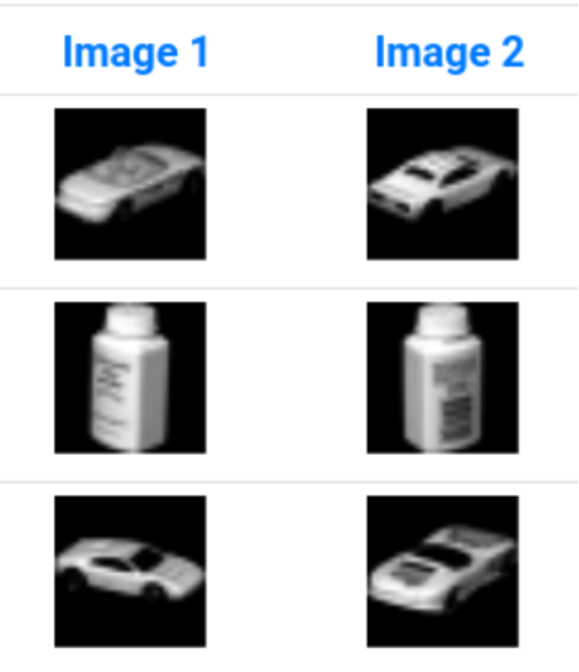
\includegraphics[width=\textwidth]{ml_examples}
        \caption{\footnotesize{Similar-link constraints.}}
    \end{subfigure}
    \begin{subfigure}[c]{0.48\linewidth}
        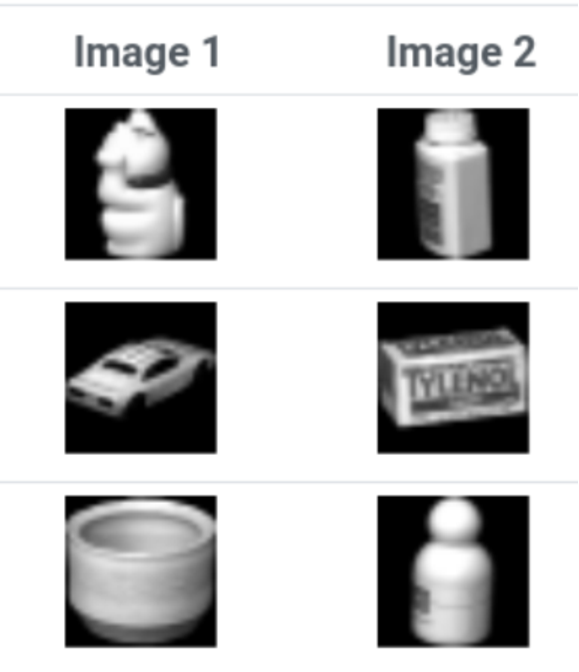
\includegraphics[width=\textwidth]{cl_examples}
        \caption{\footnotesize{Dissimilar-link constraints.}}
    \end{subfigure}
    \caption{Examples of similar-link and dissimilar-link constraints between pairs of images from COIL20 dataset (a dataset of 20 object captured under many different points of view).}
    \label{fig:ml_cl_examples}
\end{figure}

Our method is based on the hypothesis that an embedding is said to be good if it accurately represents the high-dimensional data and satisfies some given constraints.
If labels related to the dataset, which have not been used during the NLDR process, are provided, a portion of these labels can be used to generate the constraints for computing a quality score.
%This is a way to select the visualization that best fit the prior knowledge represented by the labels.
If the dataset does not contain any label, or if some particular knowledge have to be considered, constraints can directly be provided by users.
%The pairwise constraints are then used as a criterion to evaluate the fit between visualizations and user requirements. By computing this constraint score, our method makes it easier to select the NLDR hyperparameters by providing good quality embeddings that preserves the predefined constraints.

%To evaluate the reliability of the quantitative score that is derived from the pairwise constraints (defined in Section~\ref{subsec:s_score}), the score is compared with several embedding quality metrics (presented in Section~\ref{sec:result:compare}).

\subsection{Defining the Pairwise Constraints}\label{subsec:s_score}

Given a set of labeled points or user pairwise constraints, the \emph{constraint-preserving score} $f_{score}$ measures how well the pairwise constraints are preserved in a certain embedding.

\subsubsection*{Constraint Measurement}
As $t$-SNE efficiently defines links between neighboring instances, we base our constraint measurement on it. $t$-SNE uses the Student's $t$ distribution to encode the neighborhood information of the instances in the low dimensional space (see Eq.~\ref{eq:q_ij}).
The constraint-preserving score $f_{score}$ also uses a $t$ distribution in the embedded space to quantify the constraints preservation.
Let us denote the NLDR embedding result ${Y} = \{{{\bf y}_i}\}$, the set of similar-links $\mathcal{S}$ and the set of dissimilar-links $\mathcal{D}$. 
%The number of similar-link and dissimilar-link constraints are denoted by $|\mathcal{S}|$ and $|\mathcal{D}|$, respectively.
For a constrained pair of instances $({\bf y}_i, {\bf y}_j)$, the probability of ${\bf y}_i$ and ${\bf y}_j$ being neighbors is defined as
\begin{equation}\label{equ:q_link}
    q_{ij} = \frac
    { ( 1 + || {\bf y}_i - {\bf y}_j ||^2 )^{-1} }
    { \sum_{k \neq l} { ( 1 + ||{\bf y}_k - {\bf y}_l||^2 )^{-1} } }.
\end{equation}
The instances connected by a similar-link constraint are considered as neighbors and should be close in the embedding.
The instances constrained by a dissimilar-link should stay apart in the visualization, i.e. they cannot be neighbors.
Therefore, for each similar-link $({\bf y}_i, {\bf y}_j) \in \mathcal{S}$, $q_{ij}$ should be high and, inversely, $q_{ij}$ is expected to be low for each dissimilar-link $({\bf y}_i, {\bf y}_j) \in \mathcal{D}$.

\subsubsection*{Constraint-Preserving Score for Similar-Links}
The amount of similar-link information preserved in a given embedding is measured as a log-likelihood of the joint distribution of $q_{i j}$ over all similar-links $({\bf y}_i, {\bf y}_j) \in \mathcal{S}$:
\begin{equation}
f_{score}(\mathcal{S}) = \frac{1}{|\mathcal{S}|} \log \prod_{({\bf y}_i, {\bf y}_j) \in \mathcal{S}} q_{ij}
                = \frac{1}{|\mathcal{S}|} \sum_{({\bf y}_i, {\bf y}_j) \in \mathcal{S}} \log q_{ij}.
\end{equation}
If all pairs connected by similar-links are close, the log-likelihood is high and so is the $f_{score}(\mathcal{S})$.

\subsubsection*{Constraint-Preserving Score for Dissimilar-Links}
In contrast to similar-links, the probability $q_{ij}$ for each dissimilar-link $({\bf y}_i, {\bf y}_j) \in \mathcal{D}$ should be low, i.e. the log-likelihood over all dissimilar-link pairs ($\log \prod_{\mathcal{D}} q_{ij}$) must be minimized. In other words, the negative log-likelihood over all dissimilar-link constraints should be maximized. The constraint-preserving score for a set of dissimilar-links $\mathcal{D}$ is defined as
\begin{equation}
f_{score}(\mathcal{D}) = -\frac{1}{|\mathcal{D}|} \log \prod_{({\bf y}_i, {\bf y}_j) \in \mathcal{D}} q_{ij}
                = -\frac{1}{|\mathcal{D}|} \sum_{({\bf y}_i, {\bf y}_j) \in \mathcal{D}} \log q_{ij}.
\end{equation}
By maximizing $f_{score}(\mathcal{D})$, the embedding will respect the dissimilar-link constraints.
Another way to measure how well a dissimilar-link $({\bf y}_i, {\bf y}_j)$ is preserved is to use $1 - q_{ij}$. However, in practice, the value of $q_{ij}$ is very small, meaning that $1 - q_{ij}$ is close to one, which makes the log-likelihood of all dissimilar-links vanish.

\subsubsection*{Constraint-Preserving Score}

% \begin{figure}
%     \centering
%     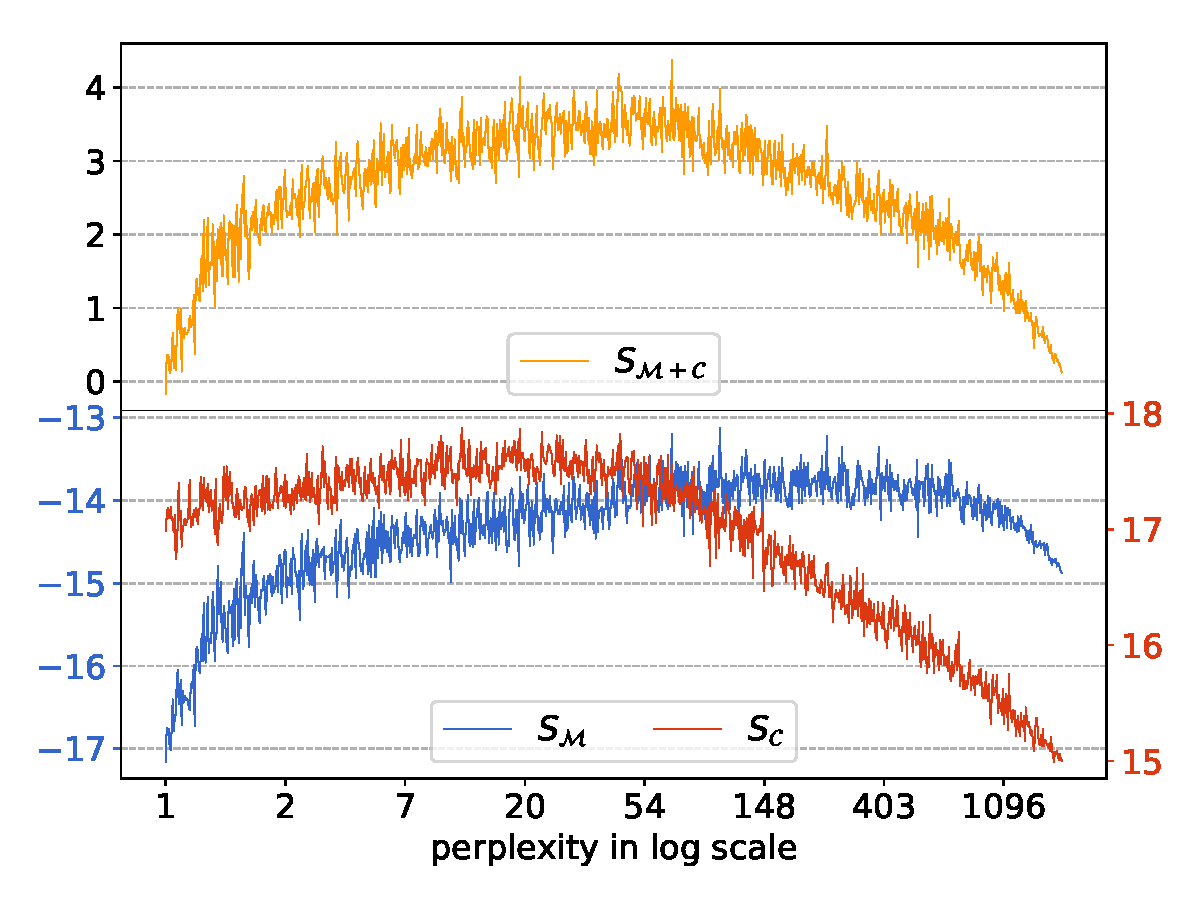
\includegraphics[width=0.85\linewidth]{s_scores_50}
%     \caption{[TODO: Replace]Evolution of constraint-preserving scores $S_{\mathcal{S}+\mathcal{D}}$, $S_{\mathcal{S}}$ and $S_{\mathcal{D}}$ with 50 constraints for $t$-SNE embeddings of \emph{DIGITS} over different perplexities.}
%     \label{fig:s_scores_mnist}
% \end{figure}

The score over all similar-constraint and dissimilar-constraint links can be defined as a combination with equal contribution of the score of both similar-links and dissimilar-links 
\begin{equation}
f_{score}(\mathcal{S},\mathcal{D}) = \frac{1}{2}f_{score}(\mathcal{S}) + \frac{1}{2}f_{score}(\mathcal{D}).
\end{equation}
$f_{score}(\mathcal{S},\mathcal{D})$ is written as $f_{score}$ for short.
An embedding that retains as much as possible the constraint information $f_{score}$ is considered to have a good quality with respect to the labels or user needs.
%Based on these definitions, our method takes a set of label- or user-defined pairwise constraints and searches, with BayOpt, among all embeddings, created by different hyperparameter values, for ones with a maximal $f_{score}$.
% Fig.~\ref{fig:s_scores_mnist} illustrates the contribution of $S_{\mathcal{S}}$ and $S_{\mathcal{D}}$ to the overall $S_{\mathcal{S}+\mathcal{D}}$ score for $t$-SNE embeddings of the \emph{DIGITS} dataset with 50 label-generated constraints (see Section~\ref{subsec:constraint_generation} for details about the generation process).

